\documentclass[article]{jss}
\usepackage[utf8]{inputenc}

\providecommand{\tightlist}{%
  \setlength{\itemsep}{0pt}\setlength{\parskip}{0pt}}

\author{
Sahir Bhatnagar *\\McGill Univeristy \And Maxime Turgeon *\\McGill University \And James Hanley\\McGill Univeristy \And Olli Saarela\\University of Toronto
}
\title{\pkg{casebase}: An Alternative Framework For Survival Analysis}

\Plainauthor{Sahir Bhatnagar *, Maxime Turgeon *, James Hanley, Olli Saarela}
\Plaintitle{casebase: An Alternative Framework For Survival Analysis}
\Shorttitle{\pkg{casebase}: An Alternative Framework For Survival Analysis}

\Abstract{
The abstract of the article. * joint co-authors
}

\Keywords{keywords, not capitalized, \proglang{Java}}
\Plainkeywords{keywords, not capitalized, Java}

%% publication information
%% \Volume{50}
%% \Issue{9}
%% \Month{June}
%% \Year{2012}
%% \Submitdate{}
%% \Acceptdate{2012-06-04}

\Address{
    Sahir Bhatnagar *\\
  McGill Univeristy\\
  1020 Pine Avenue West Montreal, QC, Canada H3A 1A2\\
  E-mail: \email{sahir.bhatnagar@mail.mcgill.ca}\\
  URL: \url{http://sahirbhatnagar.com/}\\~\\
      Maxime Turgeon *\\
  McGill University\\
  1020 Pine Avenue West Montreal, QC, Canada H3A 1A2\\
  E-mail: \email{maxime.turgeon@mail.mcgill.ca}\\
  URL: \url{http://maxturgeon.ca/}\\~\\
      James Hanley\\
  McGill Univeristy\\
  1020 Pine Avenue West Montreal, QC, Canada H3A 1A2\\
  E-mail: \email{james.hanley@mcgill.ca}\\
  URL: \url{http://www.medicine.mcgill.ca/epidemiology/hanley/}\\~\\
      Olli Saarela\\
  University of Toronto\\
  Dalla Lana School of Public Health, 155 College Street, 6th floor,
  Toronto, Ontario M5T 3M7, Canada\\
  E-mail: \email{olli.saarela@utoronto.ca}\\
  URL: \url{http://individual.utoronto.ca/osaarela/}\\~\\
  }

% Pandoc header

\usepackage{amsmath}

\begin{document}

\section{Code formatting}\label{code-formatting}

Don't use markdown, instead use the more precise latex commands:

\begin{itemize}
\tightlist
\item
  \proglang{Java}
\item
  \pkg{plyr}
\item
  \code{print("abc")}
\end{itemize}

\section{Introduction}\label{introduction}

\begin{itemize}
\tightlist
\item
  Motivation

  \begin{itemize}
  \tightlist
  \item
    Flexible
  \item
    Flexible
  \item
    Flexible
  \end{itemize}
\end{itemize}

\section{Theoretical details}\label{theoretical-details}

\section{Implementation details}\label{implementation-details}

\begin{enumerate}
\def\labelenumi{\arabic{enumi}.}
\tightlist
\item
  Population-tim plots
\item
  Sampling
\item
  Fitting
\item
  Absolute Risks
\end{enumerate}

\section{Population-time plots}\label{population-time-plots}

\section{Case study 1: Veteran data (or ERSPC if we
can)}\label{case-study-1-veteran-data-or-erspc-if-we-can}

\begin{itemize}
\tightlist
\item
  First example
\item
  Show how we can test for non-proportional hazard?
\end{itemize}

\section{Case study 2: Bone-marrow
transplant}\label{case-study-2-bone-marrow-transplant}

We will use the same data that was used in Scrucca \emph{et al}
\citep{scrucca2010regression}. The data is available on the main
author's \href{http://www.stat.unipg.it/luca/R/}{website}; it is also
available as part of this package.

\begin{CodeChunk}

\begin{CodeInput}
R> library(casebase)
\end{CodeInput}

\begin{CodeOutput}
See example usage at http://sahirbhatnagar.com/casebase/
\end{CodeOutput}

\begin{CodeInput}
R> library(magrittr)
R> library(tidyverse)
\end{CodeInput}

\begin{CodeOutput}
Loading tidyverse: ggplot2
Loading tidyverse: tibble
Loading tidyverse: tidyr
Loading tidyverse: readr
Loading tidyverse: purrr
Loading tidyverse: dplyr
\end{CodeOutput}

\begin{CodeOutput}
Conflicts with tidy packages ----------------------------------------------
\end{CodeOutput}

\begin{CodeOutput}
filter(): dplyr, stats
lag():    dplyr, stats
\end{CodeOutput}

\begin{CodeInput}
R> data(bmtcrr)
R> head(bmtcrr) %>% knitr::kable(format = "latex")
\end{CodeInput}

\begin{tabular}{l|l|l|r|r|l|r}
\hline
Sex & D & Phase & Age & Status & Source & ftime\\
\hline
M & ALL & Relapse & 48 & 2 & BM+PB & 0.67\\
\hline
F & AML & CR2 & 23 & 1 & BM+PB & 9.50\\
\hline
M & ALL & CR3 & 7 & 0 & BM+PB & 131.77\\
\hline
F & ALL & CR2 & 26 & 2 & BM+PB & 24.03\\
\hline
F & ALL & CR2 & 36 & 2 & BM+PB & 1.47\\
\hline
M & ALL & Relapse & 17 & 2 & BM+PB & 2.23\\
\hline
\end{tabular}

\end{CodeChunk}

We will perform a competing risk analysis on data from 177 patients who
received a stem cell transplant for acute leukemia. The event of
interest in relapse, but other competing causes (e.g.~transplant-related
death) need to be taken into account. We also want to take into account
the effect of several covariates such as Sex, Disease (lymphoblastic or
myeloblastic leukemia, abbreviated as ALL and AML, respectively), Phase
at transplant (Relapse, CR1, CR2, CR3), Source of stem cells (bone
marrow and peripheral blood, coded as BM+PB, or peripheral blood, coded
as PB), and Age. Below, we reproduce their Table 1:

\begin{CodeChunk}

\begin{CodeInput}
R> table1 <- tibble::tribble(
R+     ~Variable, ~Description, ~`Statistical summary`,
R+     "Sex", "Sex", "M=Male (100)",
R+     "", "", "F=Female (77)",
R+     "D", "Disease", "ALL (73)",
R+     "", "", "AML (104)",
R+     "Phase", "Phase", "CR1 (47)", 
R+     "", "", "CR2 (45)", 
R+     "", "", "CR3 (12)", 
R+     "", "", "Relapse (73)",
R+     "Source", "Type of transplant", "BM+PB (21)", 
R+     "", "", "PB (156)",
R+     "Age", "Age of patient (years)", "4–62", 
R+     "", "", "30.47 (13.04)",
R+     "Ftime", "Failure time (months)", "0.13–131.77",
R+     "", "", "20.28 (30.78)",
R+     "Status", "Status indicator", "0=censored (46)", 
R+     "", "", "1=relapse (56)", 
R+     "", "", "2=competing event (75)"
R+ )
R> 
R> knitr::kable(table1, format = "latex")
\end{CodeInput}

\begin{tabular}{l|l|l}
\hline
Variable & Description & Statistical summary\\
\hline
Sex & Sex & M=Male (100)\\
\hline
 &  & F=Female (77)\\
\hline
D & Disease & ALL (73)\\
\hline
 &  & AML (104)\\
\hline
Phase & Phase & CR1 (47)\\
\hline
 &  & CR2 (45)\\
\hline
 &  & CR3 (12)\\
\hline
 &  & Relapse (73)\\
\hline
Source & Type of transplant & BM+PB (21)\\
\hline
 &  & PB (156)\\
\hline
Age & Age of patient (years) & 4–62\\
\hline
 &  & 30.47 (13.04)\\
\hline
Ftime & Failure time (months) & 0.13–131.77\\
\hline
 &  & 20.28 (30.78)\\
\hline
Status & Status indicator & 0=censored (46)\\
\hline
 &  & 1=relapse (56)\\
\hline
 &  & 2=competing event (75)\\
\hline
\end{tabular}

\end{CodeChunk}

The statistical summary is generated differently for continuous and
categorical variables:

\begin{itemize}
\item
  For continuous variables, we are given the range, followed by the mean
  and standard deviation.
\item
  For categorical variables, we are given the counts for each category.
\end{itemize}

Note that failure time can also correspond to censoring.

In order to try and visualize the incidence density of relapse, we can
look at a population-time plot: on the X-axis we have time, and on the
Y-axis we have the size of the risk set at a particular time point.
Failure times associated to the event of interest can then be
highlighted on the plot using red dots.

\begin{CodeChunk}

\begin{CodeInput}
R> pt_object <- casebase::popTime(bmtcrr, event = "Status", time = "ftime")
R> plot(pt_object)
\end{CodeInput}


\begin{center}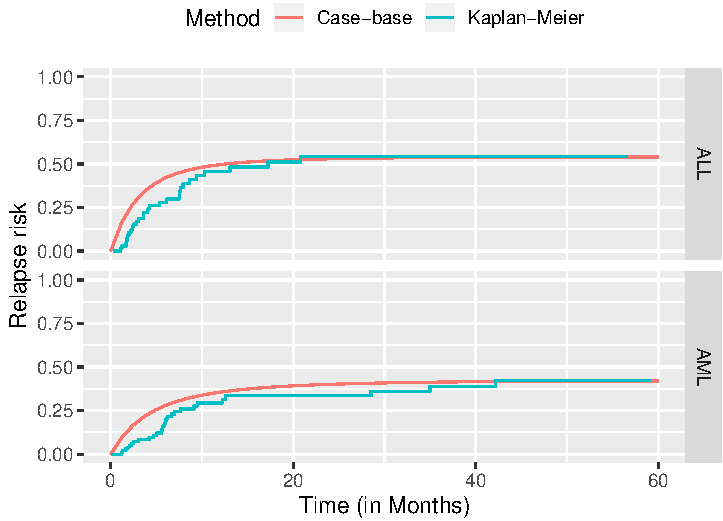
\includegraphics{casebase_jss_files/figure-latex/unnamed-chunk-3-1} \end{center}

\end{CodeChunk}

\begin{CodeChunk}

\begin{CodeInput}
R> pt_object_comp <- bmtcrr %>% 
R+     mutate(Status = case_when(Status == 1 ~ 2L, 
R+                               Status == 2 ~ 1L, 
R+                               TRUE ~ Status)) %>% 
R+     casebase::popTime(event = "Status", time = "ftime")
R> plot(pt_object_comp, point.colour = "blue")
\end{CodeInput}


\begin{center}\includegraphics{casebase_jss_files/figure-latex/unnamed-chunk-4-1} \end{center}

\end{CodeChunk}

From this last plot, we can see that there is no censoring during the
first 10 months. Moreover, we see that the last competing event occurs
around 20 months. Putting all this information together, we have
evidence of two types of patients: very sick patients who either relapse
or have a competing event early on, and healthier patients who are
eventually lost to follow-up.

We now turn to the analysis of this dataset. The population-time plots
above give evidence of non-constant hazard; therefore, we will
explicitely include time in the model. Note that we also include all
other variables as possible confounders. First, we include time as a
linear term:

\begin{CodeChunk}

\begin{CodeInput}
R> model1 <- fitSmoothHazard(Status ~ ftime + Sex + D + Phase + Source + Age, 
R+                           data = bmtcrr, 
R+                           ratio = 100,
R+                           time = "ftime")
R> summary(model1)
\end{CodeInput}

\begin{CodeOutput}

Call:
vglm(formula = formula, family = multinomial(refLevel = 1), data = sampleData)


Pearson residuals:
                       Min       1Q   Median        3Q   Max
log(mu[,2]/mu[,1]) -0.2324 -0.06980 -0.03900 -0.014615 45.18
log(mu[,3]/mu[,1]) -0.3028 -0.09008 -0.03748 -0.008052 19.79

Coefficients: 
                Estimate Std. Error z value Pr(>|z|)    
(Intercept):1  -3.473159   0.684472  -5.074 3.89e-07 ***
(Intercept):2  -2.483719   0.465134  -5.340 9.31e-08 ***
ftime:1        -0.069515   0.014754  -4.712 2.46e-06 ***
ftime:2        -0.104482   0.018274  -5.717 1.08e-08 ***
SexM:1         -0.298211   0.282266  -1.056 0.290744    
SexM:2         -0.443015   0.236317  -1.875 0.060839 .  
DAML:1         -0.580429   0.301271  -1.927 0.054029 .  
DAML:2         -0.114156   0.274610  -0.416 0.677629    
PhaseCR2:1      0.119138   0.466642   0.255 0.798485    
PhaseCR2:2      0.213409   0.331729   0.643 0.520015    
PhaseCR3:1      0.446436   0.690259   0.647 0.517783    
PhaseCR3:2      0.151515   0.526646   0.288 0.773577    
PhaseRelapse:1  1.361336   0.390162   3.489 0.000485 ***
PhaseRelapse:2  0.657054   0.307296   2.138 0.032502 *  
SourcePB:1      0.570967   0.564054   1.012 0.311415    
SourcePB:2     -0.941242   0.352134  -2.673 0.007518 ** 
Age:1          -0.008575   0.011883  -0.722 0.470504    
Age:2           0.024955   0.009868   2.529 0.011442 *  
---
Signif. codes:  0 '***' 0.001 '**' 0.01 '*' 0.05 '.' 0.1 ' ' 1

Number of linear predictors:  2 

Names of linear predictors: log(mu[,2]/mu[,1]), log(mu[,3]/mu[,1])

Residual deviance: 1412.245 on 26444 degrees of freedom

Log-likelihood: -706.1222 on 26444 degrees of freedom

Number of iterations: 10 

Reference group is level  1  of the response
\end{CodeOutput}
\end{CodeChunk}

Because of the results in Turgeon \emph{et al} \citep{turgeonCompRisk},
the standard errors we obtain from the multinomial logit fit are
asymptotically correct, and therefore can be used to construct
asymptotic confidence intervals.

From this summary, we see that time is indeed significant, as is Phase
(only relapse vs.~CR1). Interestingly, we see that the type of disease
is only significant for the event of interest, whereas the type of
transplant and the age of the patient are only significant for the
competing event.

Next, we include the logarithm of time in the model (which leads to a
Weibull hazard):

\begin{CodeChunk}

\begin{CodeInput}
R> model2 <- fitSmoothHazard(Status ~ log(ftime) + Sex + D + Phase + Source + Age, 
R+                           data = bmtcrr, 
R+                           ratio = 100, 
R+                           time = "ftime")
R> summary(model2)
\end{CodeInput}

\begin{CodeOutput}

Call:
vglm(formula = formula, family = multinomial(refLevel = 1), data = sampleData)


Pearson residuals:
                       Min       1Q   Median       3Q   Max
log(mu[,2]/mu[,1]) -0.4301 -0.06839 -0.04673 -0.03529 29.47
log(mu[,3]/mu[,1]) -0.6313 -0.07728 -0.05488 -0.04460 22.07

Coefficients: 
                Estimate Std. Error z value Pr(>|z|)    
(Intercept):1  -3.867645   0.712859  -5.426 5.78e-08 ***
(Intercept):2  -2.915708   0.470010  -6.203 5.52e-10 ***
log(ftime):1   -0.345600   0.071298  -4.847 1.25e-06 ***
log(ftime):2   -0.426302   0.057776  -7.379 1.60e-13 ***
SexM:1         -0.410838   0.293247  -1.401 0.161215    
SexM:2         -0.482041   0.243193  -1.982 0.047465 *  
DAML:1         -0.689708   0.302498  -2.280 0.022605 *  
DAML:2         -0.165629   0.285741  -0.580 0.562152    
PhaseCR2:1      0.264372   0.466874   0.566 0.571216    
PhaseCR2:2      0.389075   0.330864   1.176 0.239620    
PhaseCR3:1      0.416963   0.717569   0.581 0.561189    
PhaseCR3:2      0.035184   0.539420   0.065 0.947994    
PhaseRelapse:1  1.497807   0.391712   3.824 0.000131 ***
PhaseRelapse:2  0.900626   0.306158   2.942 0.003264 ** 
SourcePB:1      0.525555   0.606178   0.867 0.385942    
SourcePB:2     -1.129794   0.370857  -3.046 0.002316 ** 
Age:1          -0.002345   0.011604  -0.202 0.839836    
Age:2           0.029056   0.009815   2.960 0.003072 ** 
---
Signif. codes:  0 '***' 0.001 '**' 0.01 '*' 0.05 '.' 0.1 ' ' 1

Number of linear predictors:  2 

Names of linear predictors: log(mu[,2]/mu[,1]), log(mu[,3]/mu[,1])

Residual deviance: 1502.709 on 26444 degrees of freedom

Log-likelihood: -751.3548 on 26444 degrees of freedom

Number of iterations: 8 

Reference group is level  1  of the response
\end{CodeOutput}
\end{CodeChunk}

As we can see, the results are similar to the ones with a Gompertz
hazard, although Sex is now significant for the competing event.

Finally, using splines, we can be quite flexible about the way the
hazard depends on time:

\begin{CodeChunk}

\begin{CodeInput}
R> model3 <- fitSmoothHazard(
R+     Status ~ splines::bs(ftime) + Sex + D + Phase + Source + Age, 
R+     data = bmtcrr, 
R+     ratio = 100, 
R+     time = "ftime")
R> summary(model3)
\end{CodeInput}

\begin{CodeOutput}

Call:
vglm(formula = formula, family = multinomial(refLevel = 1), data = sampleData)


Pearson residuals:
                       Min       1Q   Median         3Q   Max
log(mu[,2]/mu[,1]) -0.2032 -0.07093 -0.03950 -6.478e-03 57.42
log(mu[,3]/mu[,1]) -0.2714 -0.09462 -0.01215 -3.633e-06 37.16

Coefficients: 
                        Estimate Std. Error z value Pr(>|z|)    
(Intercept):1          -3.800875   0.713833  -5.325 1.01e-07 ***
(Intercept):2          -3.255436   0.515685  -6.313 2.74e-10 ***
splines::bs(ftime)1:1   0.603866   2.311386   0.261 0.793894    
splines::bs(ftime)1:2   8.064772   3.745888   2.153 0.031321 *  
splines::bs(ftime)2:1 -17.868972   8.390698  -2.130 0.033203 *  
splines::bs(ftime)2:2 -82.148252  26.046430  -3.154 0.001611 ** 
splines::bs(ftime)3:1  -2.012019   9.340686  -0.215 0.829453    
splines::bs(ftime)3:2  -2.790995  22.345501  -0.125 0.900601    
SexM:1                 -0.277399   0.284388  -0.975 0.329349    
SexM:2                 -0.418228   0.237149  -1.764 0.077805 .  
DAML:1                 -0.649732   0.304770  -2.132 0.033017 *  
DAML:2                 -0.143387   0.278769  -0.514 0.607001    
PhaseCR2:1              0.176145   0.467658   0.377 0.706431    
PhaseCR2:2              0.340090   0.332192   1.024 0.305941    
PhaseCR3:1              0.540857   0.697533   0.775 0.438112    
PhaseCR3:2              0.241321   0.529642   0.456 0.648656    
PhaseRelapse:1          1.503814   0.395120   3.806 0.000141 ***
PhaseRelapse:2          0.874907   0.314308   2.784 0.005376 ** 
SourcePB:1              0.444475   0.576583   0.771 0.440779    
SourcePB:2             -1.174262   0.360405  -3.258 0.001121 ** 
Age:1                  -0.005234   0.011979  -0.437 0.662179    
Age:2                   0.028974   0.010077   2.875 0.004039 ** 
---
Signif. codes:  0 '***' 0.001 '**' 0.01 '*' 0.05 '.' 0.1 ' ' 1

Number of linear predictors:  2 

Names of linear predictors: log(mu[,2]/mu[,1]), log(mu[,3]/mu[,1])

Residual deviance: 1393.424 on 26440 degrees of freedom

Log-likelihood: -696.7122 on 26440 degrees of freedom

Number of iterations: 16 

Reference group is level  1  of the response
\end{CodeOutput}
\end{CodeChunk}

Again, we see that the results are quite similar for this third model.

We now look at the 2-year risk of relapse:

\begin{CodeChunk}

\begin{CodeInput}
R> linearRisk <- absoluteRisk(object = model1, time = 24, newdata = bmtcrr[1:10,])
R> logRisk <- absoluteRisk(object = model2, time = 24, newdata = bmtcrr[1:10,])
R> splineRisk <- absoluteRisk(object = model3, time = 24, newdata = bmtcrr[1:10,])
\end{CodeInput}
\end{CodeChunk}

\begin{CodeChunk}

\begin{CodeInput}
R> plot(linearRisk, logRisk,
R+      xlab = "Linear", ylab = "Log/Spline", pch = 19,
R+      xlim = c(0,1), ylim = c(0,1), col = 'red')
R> points(linearRisk, splineRisk,
R+        col = 'blue', pch = 19)
R> abline(a = 0, b = 1, lty = 2, lwd = 2)
R> legend("topleft", legend = c("Log", "Spline"),
R+        pch = 19, col = c("red", "blue"))
\end{CodeInput}


\begin{center}\includegraphics{casebase_jss_files/figure-latex/absRiskPlot-1} \end{center}

\end{CodeChunk}

We can also estimate the mean absolute risk for the entire dataset:

\begin{CodeChunk}

\begin{CodeInput}
R> mean(linearRisk)
\end{CodeInput}

\begin{CodeOutput}
[1] 0.1991813
\end{CodeOutput}

\begin{CodeInput}
R> mean(logRisk)
\end{CodeInput}

\begin{CodeOutput}
[1] 0.1560315
\end{CodeOutput}

\begin{CodeInput}
R> mean(splineRisk)
\end{CodeInput}

\begin{CodeOutput}
[1] 0.1087245
\end{CodeOutput}
\end{CodeChunk}

\begin{CodeChunk}

\begin{CodeInput}
R> # Absolute risks----
R> library(tidyverse)
R> library(magrittr)
R> library(splines)
R> library(survival)
R> library(timereg)
R> 
R> bmtcrr %<>% filter(Age >= 16)
R> 
R> bmtcrr %>% select(Sex) %>% table
\end{CodeInput}

\begin{CodeOutput}
.
 F  M 
72 87 
\end{CodeOutput}

\begin{CodeInput}
R> bmtcrr %>% select(D) %>% table
\end{CodeInput}

\begin{CodeOutput}
.
ALL AML 
 59 100 
\end{CodeOutput}

\begin{CodeInput}
R> bmtcrr %>% select(Phase) %>% table
\end{CodeInput}

\begin{CodeOutput}
.
    CR1     CR2     CR3 Relapse 
     44      40      10      65 
\end{CodeOutput}

\begin{CodeInput}
R> bmtcrr %>% select(Source) %>% table
\end{CodeInput}

\begin{CodeOutput}
.
BM+PB    PB 
   15   144 
\end{CodeOutput}

\begin{CodeInput}
R> bmtcrr %>% select(Status) %>% table
\end{CodeInput}

\begin{CodeOutput}
.
 0  1  2 
40 49 70 
\end{CodeOutput}

\begin{CodeInput}
R> model_cb <- fitSmoothHazard(Status ~ bs(ftime, df = 5) + Sex + D + Phase + Source + Age,
R+                             data = bmtcrr, time = "ftime")
R> model_fg <- comp.risk(Event(ftime, Status) ~ const(Sex) + const(D) + 
R+                           const(Phase) + const(Source) + const(Age), 
R+                       data = bmtcrr, cause = 1, model = "fg")
R> model_cox <- coxph(Surv(ftime, Status == 1) ~ Sex + D + Phase + Source + Age,
R+                    data = bmtcrr)
R> 
R> time_points <- (0:100)*60/100
R> 
R> # ALL vs. AML
R> newdata <- data.frame("Sex" = factor(c("F", "F"), 
R+                                      levels = c("F", "M")),
R+                       "D" = c("ALL", "AML"),
R+                       "Phase" = factor(c("Relapse", "Relapse"), 
R+                                        levels = c("CR1", "CR2", "CR3", "Relapse")),
R+                       "Age" = c(35, 35),
R+                       "Source" = factor(c("PB", "PB"), 
R+                                         levels = c("BM+PB", "PB")))
R> 
R> risk_cb <- absoluteRisk(object = model_cb, time = time_points,
R+                         method = "montecarlo", newdata = newdata)
R> risk_cb <- bind_rows(data.frame(Time = time_points, Method = "Case-base", Risk = risk_cb[,2], Disease = "ALL",
R+                                 stringsAsFactors = FALSE),
R+                      data.frame(Time = time_points, Method = "Case-base", Risk = risk_cb[,3], Disease = "AML",
R+                                 stringsAsFactors = FALSE))
R> 
R> risk_fg <- predict(model_fg, newdata, times = time_points)
R> risk_fg <- bind_rows(data.frame(Time = time_points, Method = "Fine-Gray", Risk = risk_fg$P1[1,], Disease = "ALL",
R+                                 stringsAsFactors = FALSE),
R+                      data.frame(Time = time_points, Method = "Fine-Gray", Risk = risk_fg$P1[2,], Disease = "AML",
R+                                 stringsAsFactors = FALSE))
R> risk_km <- map_df(c("ALL", "AML"), function(disease) {
R+     foo <- bmtcrr %>% 
R+         filter(D == disease) %>% 
R+         survfit(Surv(ftime,Status == 1) ~ 1, data = .)
R+     data.frame(Time = foo$time, Method = "Kaplan-Meier", Risk = 1 - foo$surv, Disease = disease,
R+                stringsAsFactors = FALSE) %>%
R+         filter(Time <= 60)
R+ })
R> 
R> disease_names <- c("ALL" = "Acute Lymphoid Leukemia",
R+                    "AML" = "Acute Myeloid Leukemia")
R> risk_cb %>%
R+     bind_rows(risk_fg,
R+               risk_km) %>% 
R+     arrange(Disease, Risk) %>% 
R+     ggplot(aes(Time, Risk, colour = Method)) + 
R+     geom_line(data = . %>% filter(Method == "Case-base")) + 
R+     geom_step(data = . %>% filter(Method != "Case-base")) + 
R+     facet_grid(Disease ~ ., labeller = as_labeller(disease_names)) + ylim(c(0,1)) +
R+     theme(legend.position = "top") +
R+     xlab("Time (in Months)") + ylab("Relapse risk")
\end{CodeInput}


\begin{center}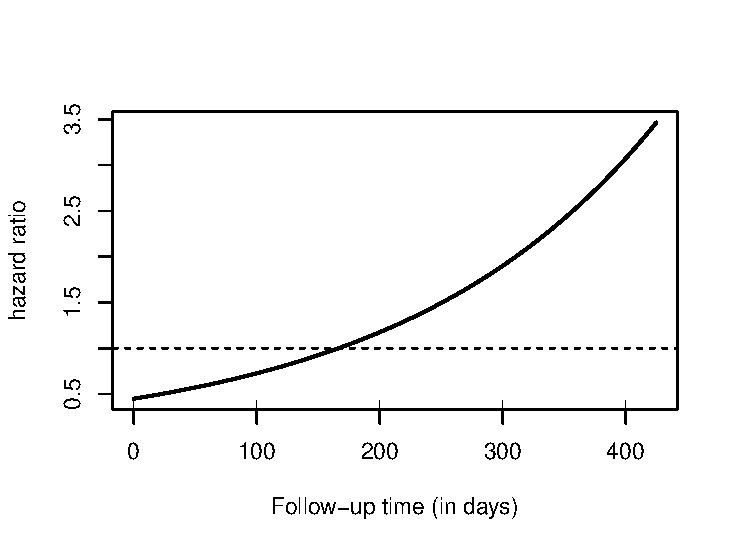
\includegraphics{casebase_jss_files/figure-latex/unnamed-chunk-9-1} \end{center}

\end{CodeChunk}

\textbackslash{}begin\{CodeChunk\}

\textbackslash{}begin\{CodeInput\} R\textgreater{} \# Table of
coefficients---- R\textgreater{} z\_value \textless{}- qnorm(0.975)
R\textgreater{} table\_cb \textless{}- summary(model\_cb)\citet[seq(13,
25, by = 2), 1:2]{coef3} R\textgreater{} table\_cb \textless{}-
cbind(table\_cb{[},1{]}, R+ table\_cb{[},1{]} - z\_value *
table\_cb{[},2{]}, R+ table\_cb{[},1{]} + z\_value * table\_cb{[},2{]})
R\textgreater{} table\_cb \textless{}- round(exp(table\_cb), 2)
R\textgreater{} R\textgreater{} table\_cox \textless{}-
round(summary(model\_cox)\$conf.int{[},-2{]}, 2)
\textbackslash{}end\{CodeInput\} \textbackslash{}end\{CodeChunk\}

\section{Case study 3: Vaccination study (recurrent
events)}\label{case-study-3-vaccination-study-recurrent-events}

\begin{itemize}
\tightlist
\item
  Give a more complex example of sampling; time-dependent exposure

  \begin{itemize}
  \tightlist
  \item
    Sampling needs to be done manually, but fitting function can still
    be used
  \end{itemize}
\end{itemize}

\section{Discussion}\label{discussion}

\section*{References}\label{references}
\addcontentsline{toc}{section}{References}

\bibliography{casebase_references.bib}


\end{document}

